%TODO:


\documentclass{scrartcl}


\usepackage[utf8]{inputenc}
\usepackage[english]{babel}
\usepackage{lmodern} 
\usepackage[T1]{fontenc}
\usepackage{booktabs}
\usepackage{multirow}
\usepackage{wrapfig}


% PAKETE
\usepackage{siunitx}
\usepackage{graphicx}
\usepackage[usenames,dvipsnames,table]{xcolor}
\usepackage{placeins}
\usepackage{longtable}
\usepackage{enumitem}
\usepackage{bbm}

\usepackage{amssymb} % math symbols
\usepackage{amsmath} % ams
\usepackage{amsfonts} % mathmatical fonts

% caption indenting
 \usepackage[format=plain,indention=0em,labelfont=bf,margin=1em]{caption} 
 \usepackage{subfig} %subfigures ^^
\usepackage[protrusion=true,expansion=true]{microtype} % denser font, "-" behind line
\usepackage{esint} % nicer double and triple integrals
\usepackage{fancyhdr} % fancy headers
\usepackage[colorlinks=true,linkcolor=black,citecolor=black,filecolor=black,urlcolor=black]{hyperref}



% EINSTELLUNGEN
\sisetup{seperr,repeatunits=false}
\numberwithin{equation}{section}
\numberwithin{figure}{section}
\numberwithin{table}{section}

% EIGENE FUNKTIONEN
\newcommand{\re}{\operatorname{Re}}
\newcommand{\im}{\operatorname{Im}}
\newcommand{\gquote}[1]{\glqq #1 \grqq}

\newcommand{\eq}[2]{\begin{equation}#1\label{#2}\end{equation}}
\newcommand{\eqand}[0]{\hspace{.25cm} \bigwedge \hspace{.25cm}}
\newcommand{\grafik}[2]{\begin{figure}[h]\centering \includegraphics[width=10cm]{#1.eps}  \caption{#2} \label{#1} \end{figure} }
\newcommand{\grafikq}[3]{\begin{figure}[h]\centering \includegraphics[width=10cm]{#1.eps}  \caption[#2]{#3} \label{#1} \end{figure} }
\newcommand{\tbl}[3]{\begin{table}[h]\caption{#1}\label{#2}\begin{center}#3\end{center}\end{table}}
\newcommand{\Abbildung}[1]{\textsl{Abbildung \ref{#1}}}
\newcommand{\AbbildungI}[1]{\textsl{(Abbildung \ref{#1})}}
\newcommand{\Tabelle}[1]{\textsl{Tabelle \ref{#1}}}
\newcommand{\TabelleI}[1]{\textsl{(Tabelle \ref{#1})}}
\newcommand{\Formel}[1]{(\ref{#1})}
\renewcommand{\d}{\mathrm{d}}
\newcommand{\ve}[1]{\mathbf{ #1} }

\title{Ma 5: Dynamical Processes in Lipid Membranes}
\subtitle{Tutor: Dr. P. Chernev}
\author{Benjamin Huber, Carolin Wille}
\date{January 30, 2012}

\begin{document}
\thispagestyle{empty}
\maketitle
\tableofcontents
\clearpage

\section{Introduction}
A common method for observation of a biophysical system is the measurement of phosphorescence. The added phosphorescent molecules react specifically depending on the temperature, surrounding molecules (lipophil or hydrophil?), PH value and so on, allowing a spatially resolved picture of the sample conditions. While the spatial resolution is often of special interest (especially if the phosphorescent molecules are specifically attached to other molecules of the system), we will concentrate on the temporal evolution of phosphorescence, their polarity and dependence on the temperature.


\subsection{Fluorescence and Absorption spectra}
\subsubsection{Dipole Transitions and the Franck-Condon Principle}
In order to understand the emission and absorption spectrum of molecules, it is important to know the structure of energy levels and the transitions, which can occur between them. In the Born-Oppenheimer approximation, which is valid if the electronic transitions happen on a much shorter time scale than the changes in the distance of the atomic nuclei, the wavefunction, which describes the state of the molecule factorises in electronic and nuclear components. The components connected to the nuclei include rotation and vibrational states. If the rotational degrees of freedom are suppressed, e.g. if the molecule is embedded in a certain structure, only the vibrational levels are relevant. The transitions, which lead to the emission of visible light are electronic transitions, that are combined with a vibronic transition. In the dipole approximation, that is valid if the wavelength of the emitted light is considerably longer than the atomic radii, the probability amplitude for such an electronic-vibronic transition is given by the matrix elements of the final and initial states $\Psi,\Psi'$ with the dipole operator $\ve {\hat{D}}$
\eq{ P = \langle \Psi'  \mid   \ve {\hat{D}} \mid \Psi \rangle =  \langle \psi_\text{el'} \mid   \ve {\hat{D}_{el}} \mid \psi_\text{el} \rangle \langle \psi_\text{s'} \mid \psi_\text{s} \rangle \langle \psi_\nu'  \mid  \psi_\nu \rangle \; .} {transition }
The spatial overlap of the two vibronic state nuclear wavefunction squared  $\lvert \langle \psi_\nu'  \mid  \psi_\nu \rangle \rvert ^2$ is called the Franck-Condon factor and expresses the fact, that transitions are more likely to occur, if the position of the nuclei remain more or less the same during an electronic transition. This is called the Franck-Condon principle and is illustrated in figure \ref{condon}. 
The direction of the dipole operator gives the polarization direction of the photons, which are absorbed or emitted.
Considering two electronic states with similar vibronic structure, the absorption spectrum is symmetric to the fluorescence spectrum as a consequence of the Franck-Condon principle (cf. \ref{condon}). This symmetry can be detected in the experiment although the equal spacing of the energy levels is an idealization, meaning that the real structures do not look exactly symmetric.

\begin{figure}
\centering
\subfloat[][Franck-Condon Principle]{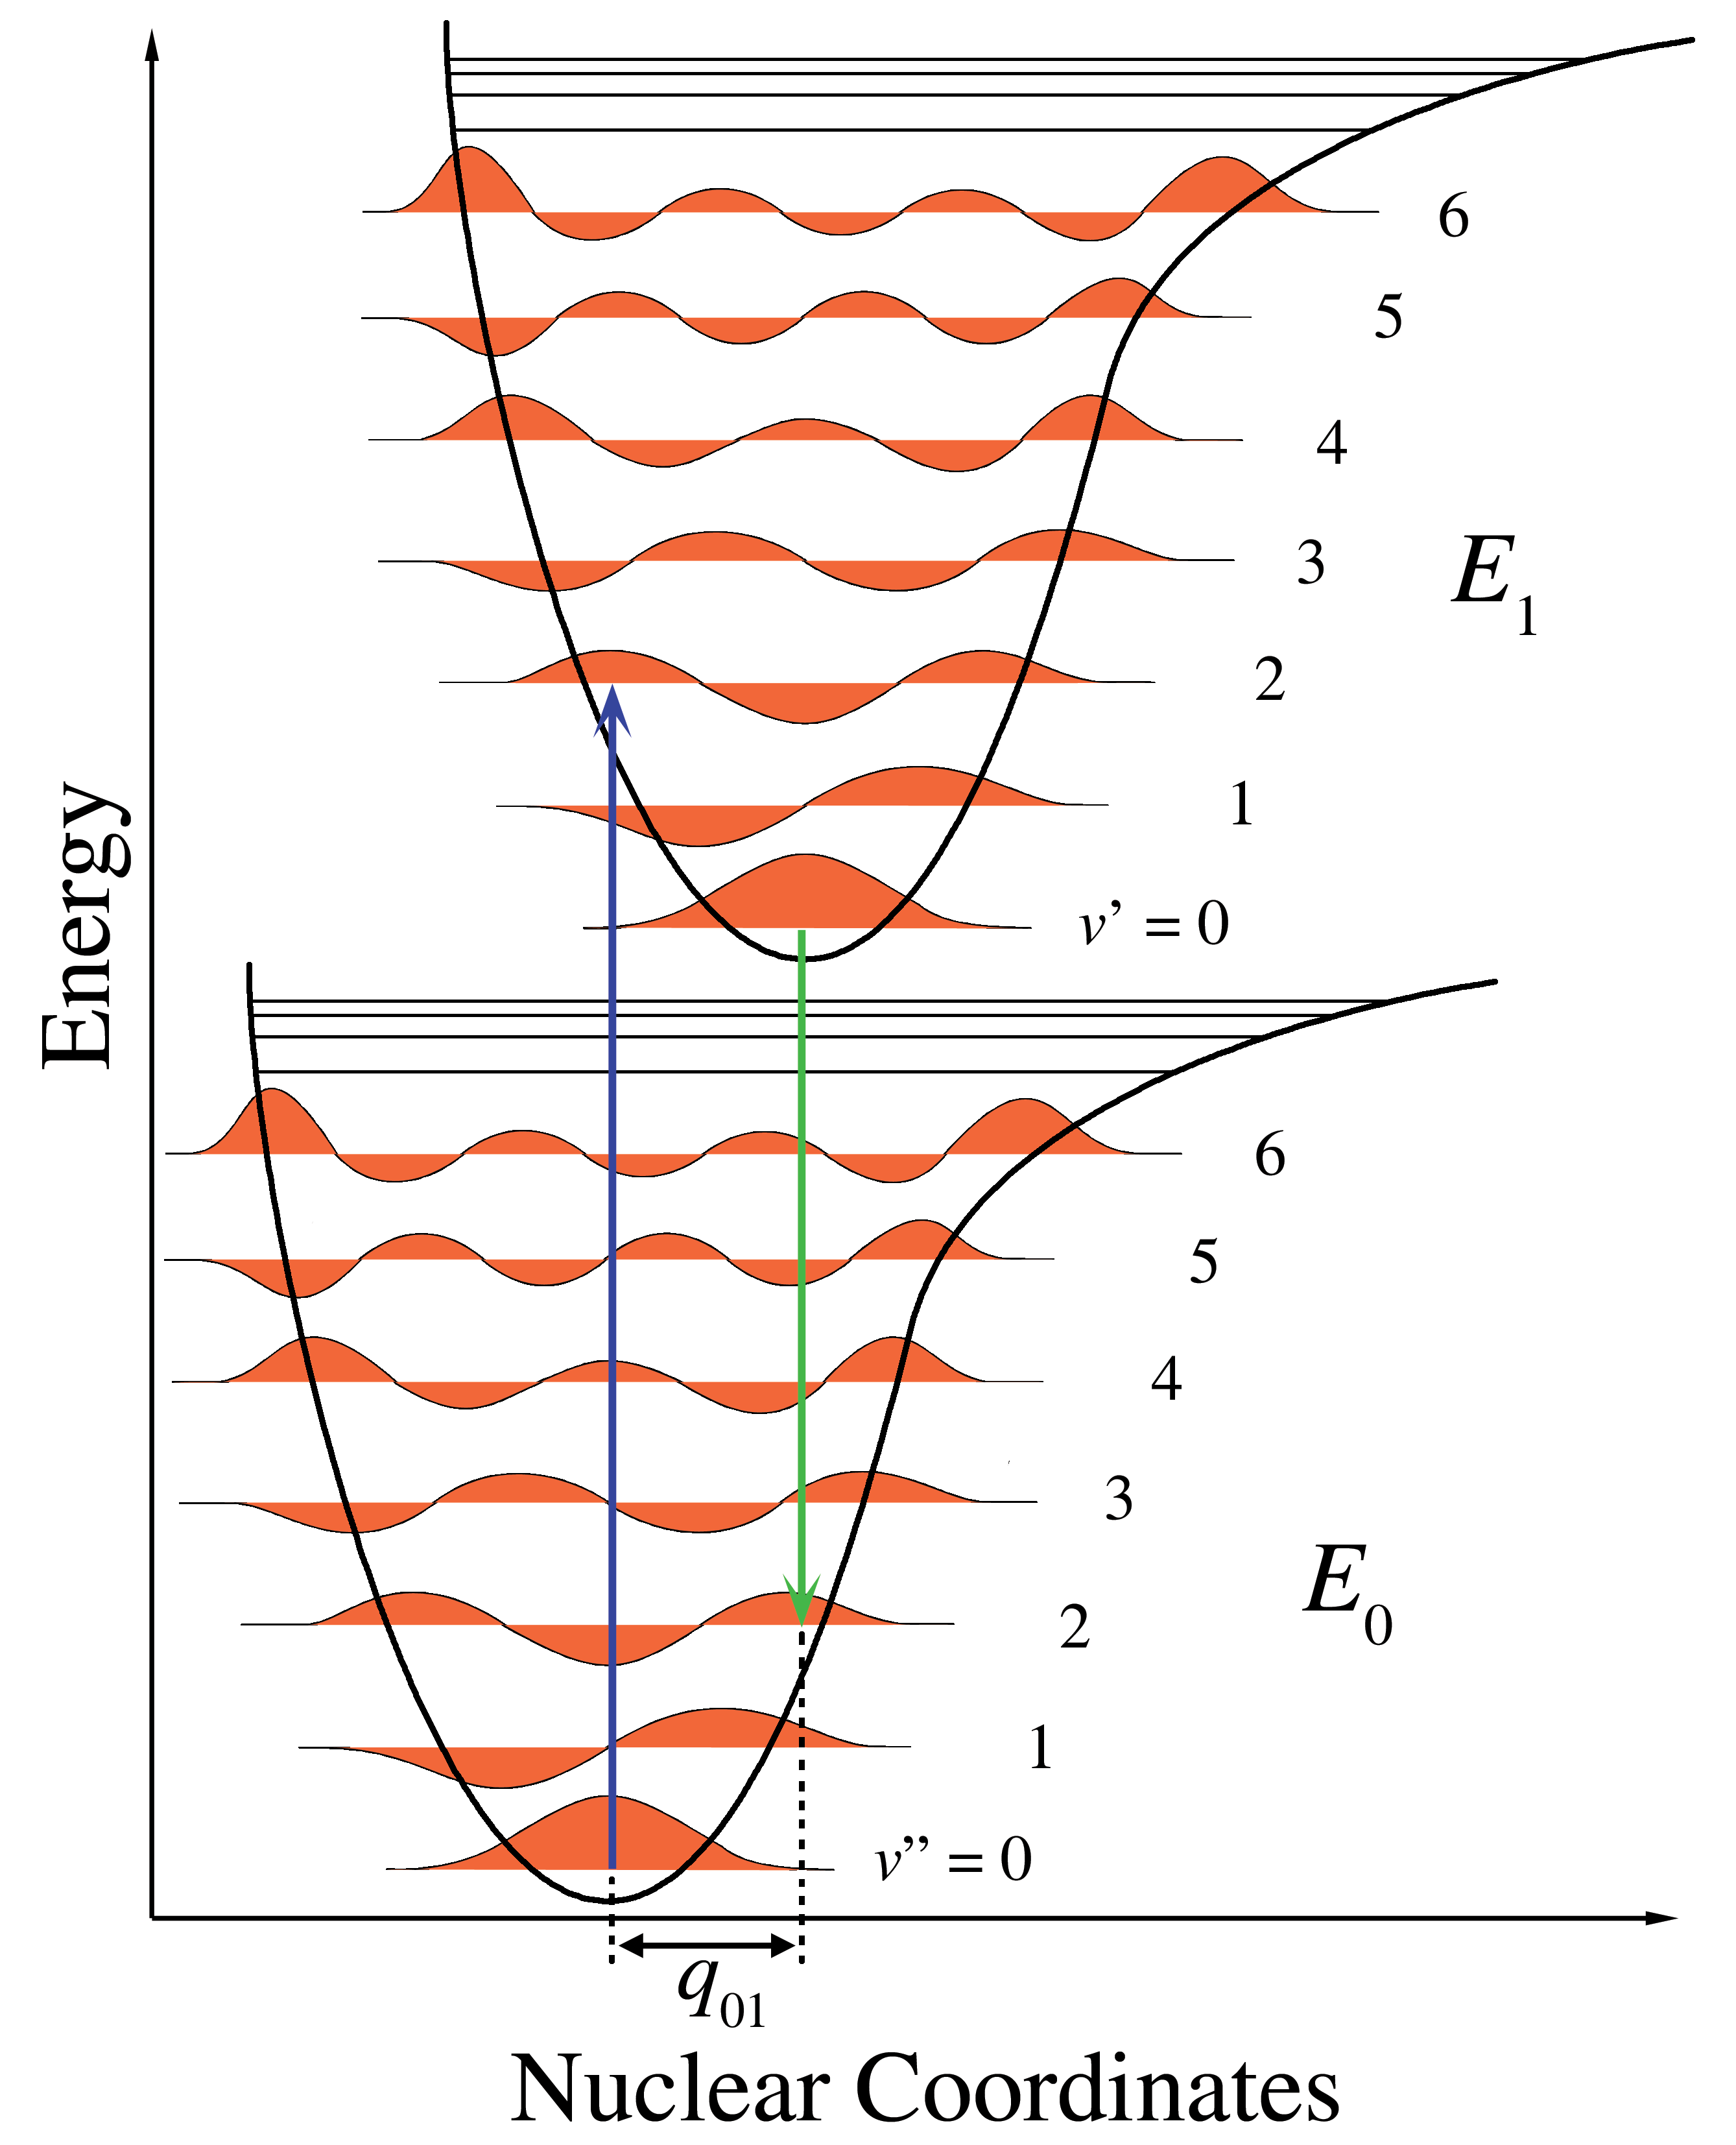
\includegraphics[width=0.5\linewidth]{img/condon.png}}
\hfill
\subfloat[][Spectrum]{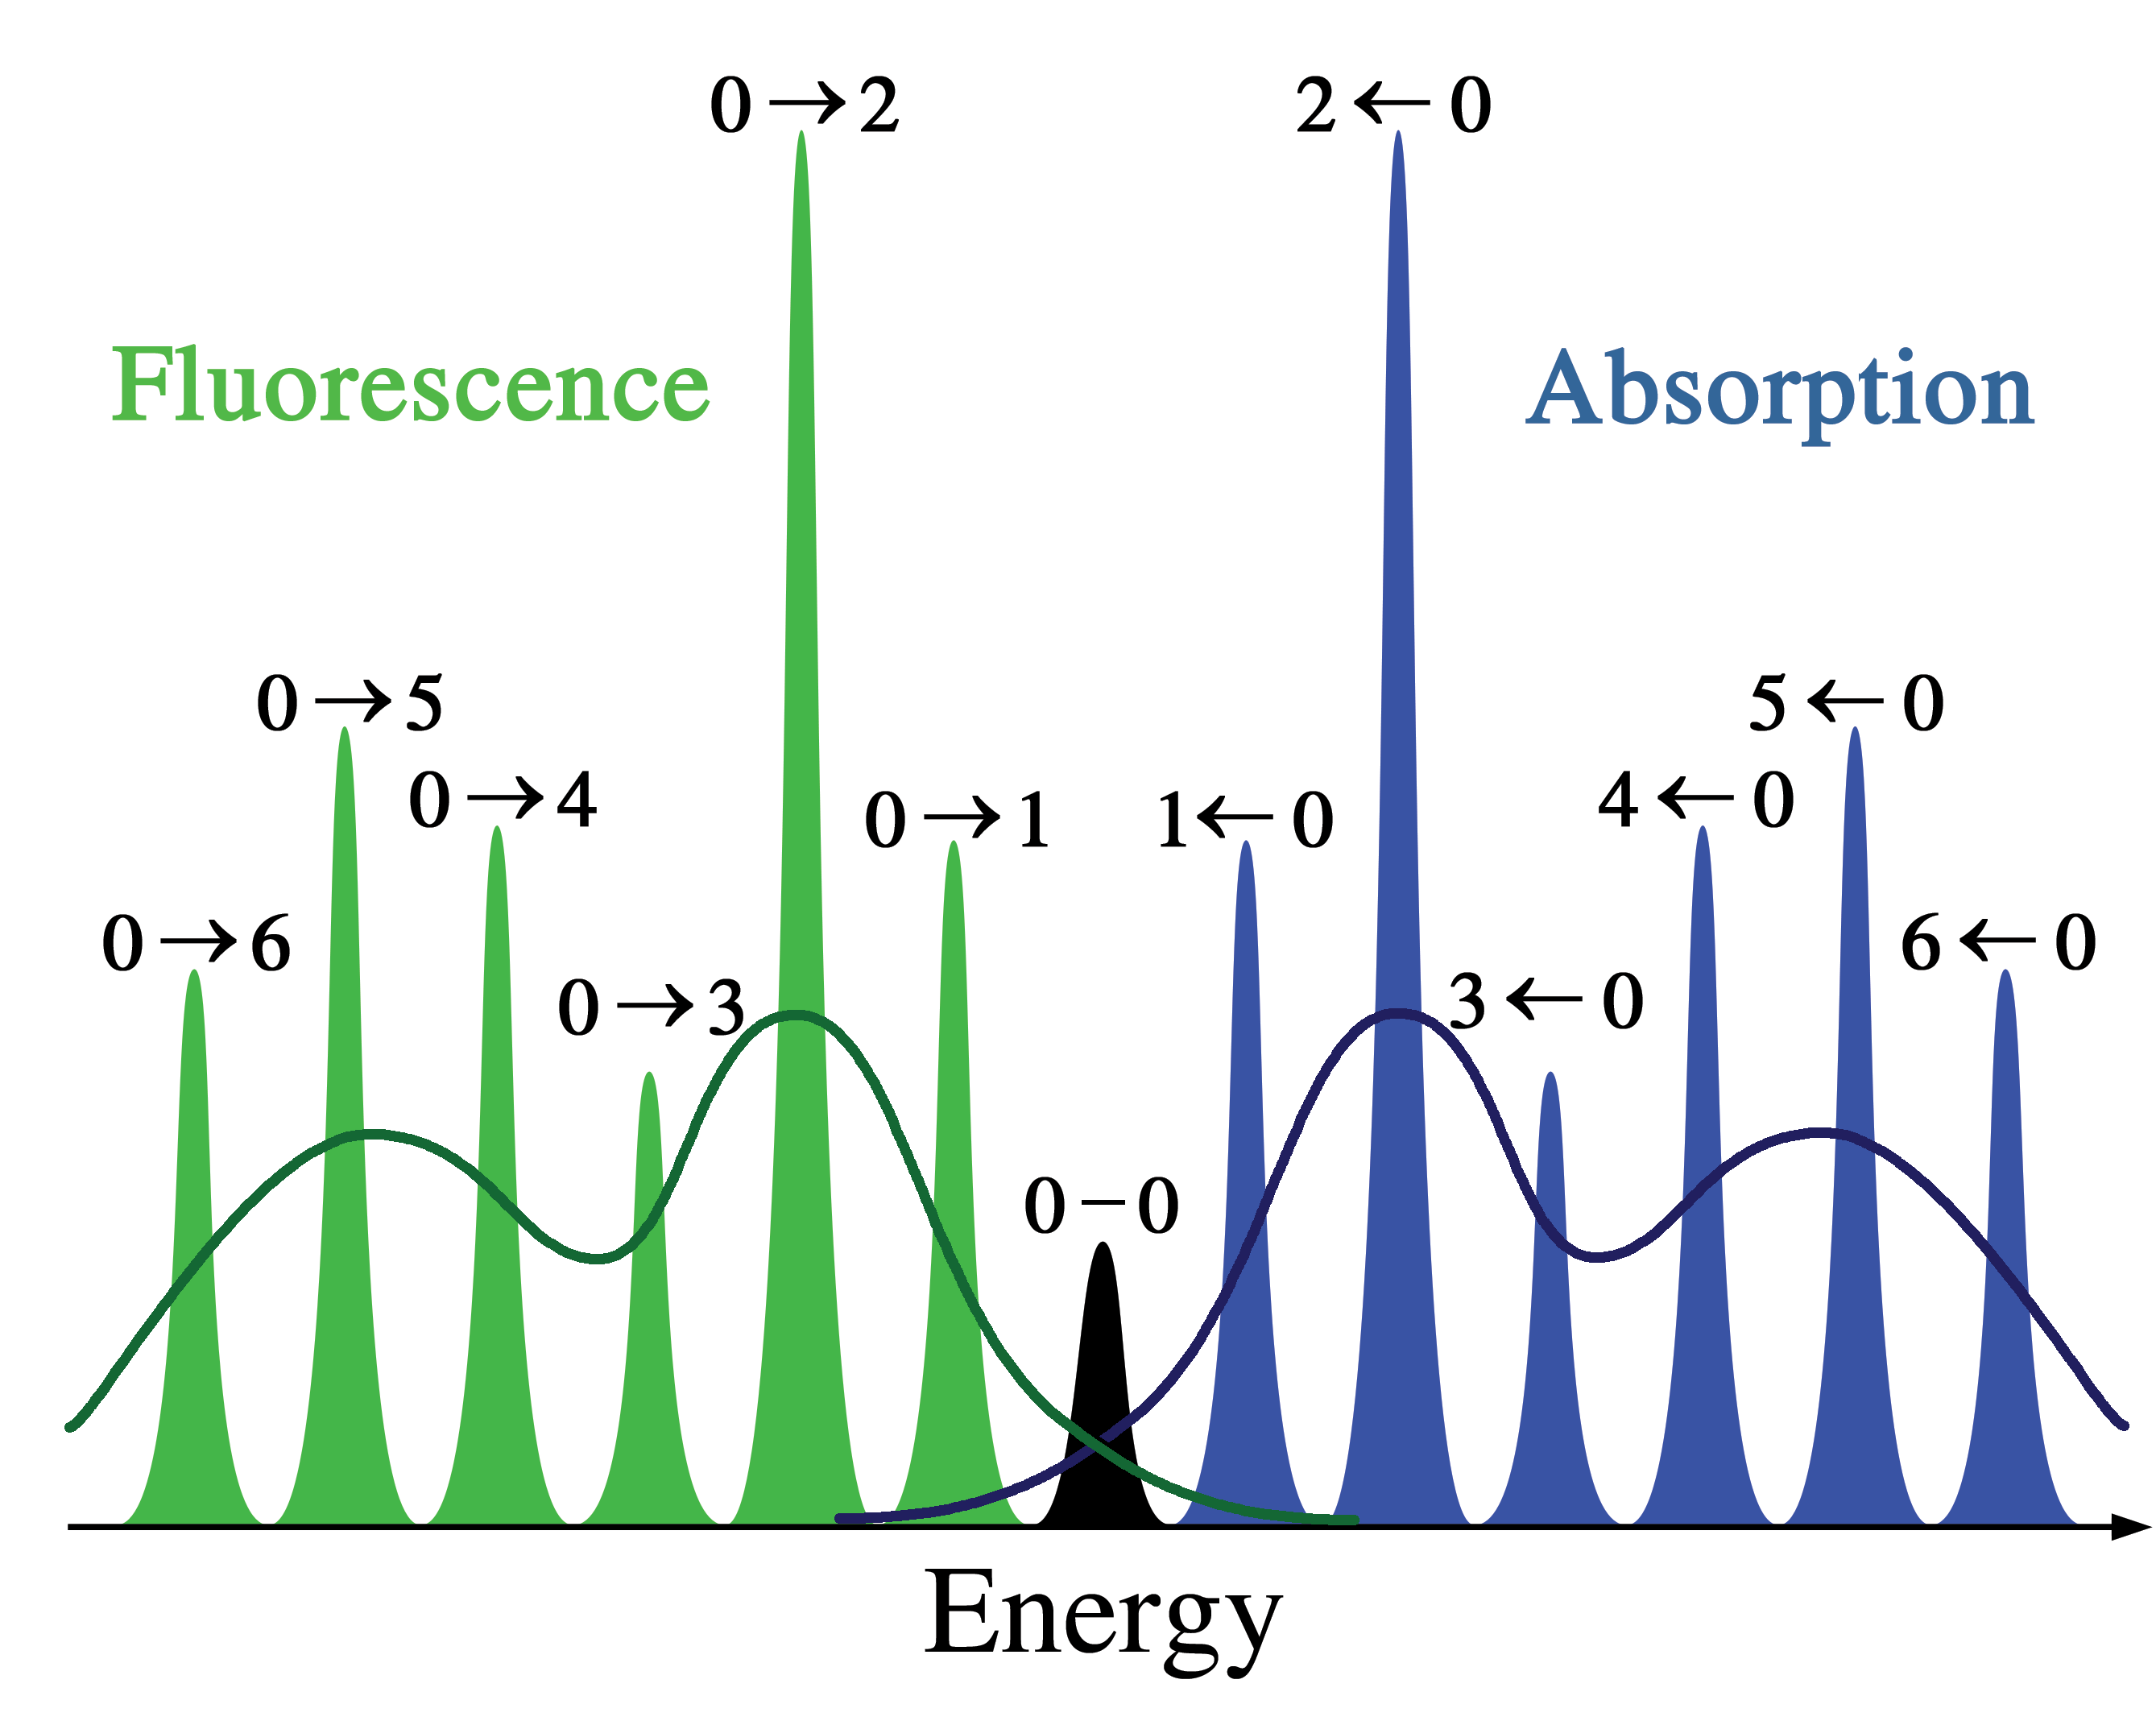
\includegraphics[width=0.5\linewidth]{img/absorptionemission.png}}

\subfloat[][Jablonski Diagram]{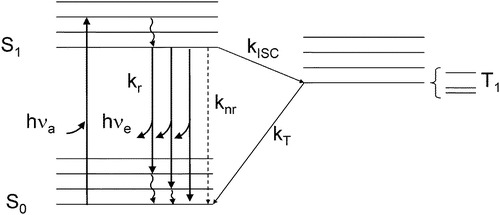
\includegraphics[width=0.7\textwidth]{img/Jablonski.jpg}}
\caption{ \small \textbf{(a)} Illustration of the Franck-Condon principle, which is a direct consequence of the Born-Oppenheimer approximation and states, that those electronic-vibraonic transitions are favored, which leave the inter-nuclei distance mostly unchanged. 
\textbf{(b)} Symmetric structure of an absorption and fluorescence spectrum. Sharp peaks will be visible in dilute gases, while in liquids and solids the peaks are widened. 
\textbf{(c)} Jablonski Diagram of different relaxation processes. ISC denotes intersystem crossing. $K_T$ the relaxation via phosphorescence. $K_r$ denotes fluorescence and $K_{nr}$ radiationless transitions, which also reduce the fluorescence lifetime. \footnotesize Source: \textbf{(a)}, \textbf{(b)} \url{http://en.wikipedia.org/wiki/Franck-Condon_principle}, \textbf{(c)} \cite{omg}}
\label{condon}
\end{figure}

\begin{figure}
\centering
\subfloat[][DPH Molecule]{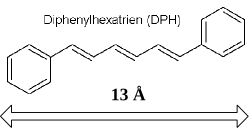
\includegraphics[width=0.5\linewidth]{img/dph.png}}
\subfloat[][Lipid Membrane]{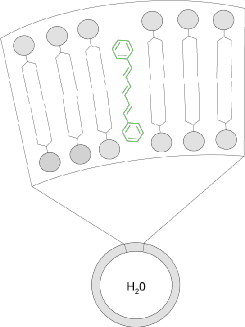
\includegraphics[width=0.35\linewidth]{img/membrane.png}}
\caption{ \small \textbf{(a)}Diphenylhexatriene (DPH) molecule, which is used as a reporter molecule in the lipid membrane. \textbf{(b)} Lipid membrane vesicle with a close-up of the bilayer, where a DPH molecule is embedded.}
\label{dph}
\end{figure}

\subsubsection{Relaxation Processes}
An excited state can relax into its groundstate via different intermediate processes. Radiation less transitions, which can occur via exchange of phonons or collisions with other atoms and molecules are usually very fast, because the energy difference between those states is typically small. Thus, an excited vibronic state decays fast into its ground state. The relaxation of the electronic excited state and vibronic ground state into the electronic ground state and excited vibronic state (cf. fig \ref{condon} \textbf{(c)}) is called fluorescence. As its emitted photons are typically in the visible light regime, fluorescence is a luminescent process. The other luminescence, which can occur is phosphorescence, where the system decays first into a state, which is forbidden according to spin selection rules. Such a transition, where the electron spin changes is called intersystem crossing. The decay into ground state is again forbidden according to the dipole selection rules. Therefore, the lifetime if this state is very high, which leads to the phenomenon of light emission long after absorption.

Another process is the so called fluorescence quenching, where the fluorescence is suppressed by the transition of energy to certain molecules. For the molecule used in the experiment, water acts as a quenching molecule and reduces the fluorescence intensity to $1/200$ of the value in hydrophobic media like the interior of lipid membrane bilayers.

The fluorescence lifetime $\tau_f$ is defined as the inverse of the decay rate $k_f$, which characterises the exponential decay of the excited state via fluorexcence
\eq{N(t) =N_0 \exp (-k_f \cdot  t) , \qquad \tau_f=1/k_f \; .}{rate}
The quantum yield $\Phi$ relates the total lifetime of the excited level $\tau$ to the fluorescence life time $\tau = \tau_f \Phi$. It is defined as the number of emitted photons divided by the number of absorbed photons. In terms of the different decay rates, it reads
\eq{\Phi = \frac{N_\text{em}}{N_\text{abs}} = \frac{k_f}{k_f +k_{ic} + k_{isc} + k_Q} \; ,}{yield}
where $k_{ic}$ and $k_{isc}$ denote internal converstion and intersystem crossing and $k_Q$ the quenching rate.



\subsubsection{Specifications to Fluorophores}
In heterocyclic and aramoatic molecules, which are called fluorophores, the ground state is given, when the electrons are both in bonding $\pi$ orbitals. They have antiparallel spins leading to total spin zero, which is referred to as a singulet state S$_{0,\pi\pi}$. The first excited electronic state is then a state, where one electron is in the antibonding $\pi^*$ orbital. In this excited state, the electrons can have parallel or antiparallel spin leading to singulet S$_{1, \pi \pi^*}$ and triplet states T$_{1, \pi \pi^*}$. The triplet states have usually lower energy.

In this experiment the fluorophore Diphenylhexatriene (DPH) is used as a reporter probe, which is embedded in to the lipid membrane (cf. fig. \ref{dph}).




\subsection{Rotational Diffusion}
After excitation with a polarized photon, the dipole moment is most probably aligned into the direction of the polarization. A photon emitted directly after excitation would then have the same polarization. However, as a certain time passes between excitation and radiative relaxation, the molecule can rotate in the mean time, which leads to a shift of the polarization. This rotational diffusion leads to the relaxation into an equilibrium state, which is completely isotropic unless certain symmetries are broken. The decay rate of this relaxation and the final state both give information about the degrees of freedom of the molecule and thus also about the environment of the molecule. A simple quantity to measure the rotational anisotropy is defined by
\eq{R=\frac{I_\parallel -I_\perp}{I_\parallel+ 2I_\perp} \; ,}{R}
where $I_{\parallel,\perp }$ are given by
\eq{I_\parallel = \frac{I_\text{VV}}{I_\text{HV}} , \qquad I_\perp = \frac{I_\text{VH}}{I_\text{HH}} \; , }{idef}
and e.g. $I_{HV}$ denotes the intensity of the fluorescent light, that was excited with light polarized horizontally and emitted with  polarization (measured with the use of a vertical polarization filter). This formula is identical to the one used by Lackowicz \cite{lako}
\eq{R=\frac{I_{VV} - G I_{VH}}{I_{VV}+ 2 G I_{VH}} \; ,}{Ralt}
where $G$ is given by $G=I_{HV}/I_{HH}$.

The rotational diffusion can be expressed by a diffusion constant \cite{heyn}
\eq{ D = \frac{1-R(\infty)/R(0)}{6\Phi_\text{rot}} = \frac{k_B T}{8\pi \eta V_\text{eff} f} }{eq:diff}
where $\Phi_\text{rot}$ is the mean rotational correlation time, $k_B$ the Boltzmann constant, $V_\text{eff}$ the effective volume, $\eta$ the viscosity and $f$ the shape factor of the radiating molecule.

\subsection{Wobbing in Cone Model}
The movement of an DPH molecule in a membrane can be described by the Wobbing in Cone model. This model assumes, that the orientation of the molecule is confined to a cone of opening angle $\theta$ and may fluctuate within this cone (``wobbing''). According to this model the ratio of the anisotropy limits is related to the opening angle by
\eq{ \frac{R(\infty)}{R(0)} = \left[ 0.5 \cos \theta (1+\cos \theta) \right]^2 }{}
\eq{ \Rightarrow \theta = \arccos \left[ 0.5\left( \sqrt{1+8\sqrt{R(\infty)/R(0)}}-1 \right) \right] }{eq:theta}

\subsection{Phase Transition}
Obviously the mobility of the membrane and thus the anisotropy is dependant on the temperature $T$. The plot of $R(T)$ is not a linear (or other simple) function though, but presents a steep change between two linear functions at a critical temperature $T_C$. This corresponds to a phase transition in the membrane between a phase of two dimensional liquid crystals and gel like phase.

To describe the steep change between the two phases further consider the equilibrium with particle numbers $M_1=M_2$. The equilibrium constant can be written as
\eq{K = \frac{M_2}{M_1} = K_0 e^{\frac{\delta H}{R T}}}{K}
\eq{\Rightarrow \frac{d}{dT}(\ln K) = \frac{\delta H}{R T}}{dK}
where $R$ is the universal gas constant and $\delta H$ the change in enthalpy. This last equation is called the van't Hoff equation. The degree of transformation or conversion yield 
\eq{\Theta = \frac{M_2}{M_1+M_2}}{Theta}
together with equation \ref{dK} allows for the determination of $\delta H$ in terms of the change of $\Theta$ at the critical temperature $T_C$ where $M_1=M_2$
\eq{{\left.\frac{d\Theta}{dT}\right |}_{T_C} = \frac{\delta H}{4 R T^2} .}{dTheta}

\clearpage
~
\clearpage

\section{Experiment}
All measurements are performed with the set-ups shown in figure \ref{fig:setup}, that include one set-up for steady-state fluorescence measurements and one for time-resolved measurements. The steady-state set-up consists of a high pressure xenon lamp as light source, followed by a monochromator, that can be driven automatically, a polarization filter and a semi reflecting semi transmitting mirror, which splits the light ray. One ray passes an aperture and than hits a reference sample, the reflected intensity is measured with a photomultiplier (PM1) and is used divide out changes in the optical setup, which have nothing to do with the real measurement. The other part of the ray passes a lens and then hits the sample. The light emitted in a $90 \degree$ angle passes another lens, an aperture, a second polarization filter and a monochromator, which can also be driven automatically before being detected by another photomultiplier (PM2).

The time-resolved set-up is similar, despite the fact, that a flash lamp is used instead of the xenon lamp and no reference sample is included in the setup. Furthermore, the monochromators are removed and a high pass filter is inserted in front of the photomultiplier.

\begin{figure}[h]
\centering
\subfloat[][Static Set-Up]{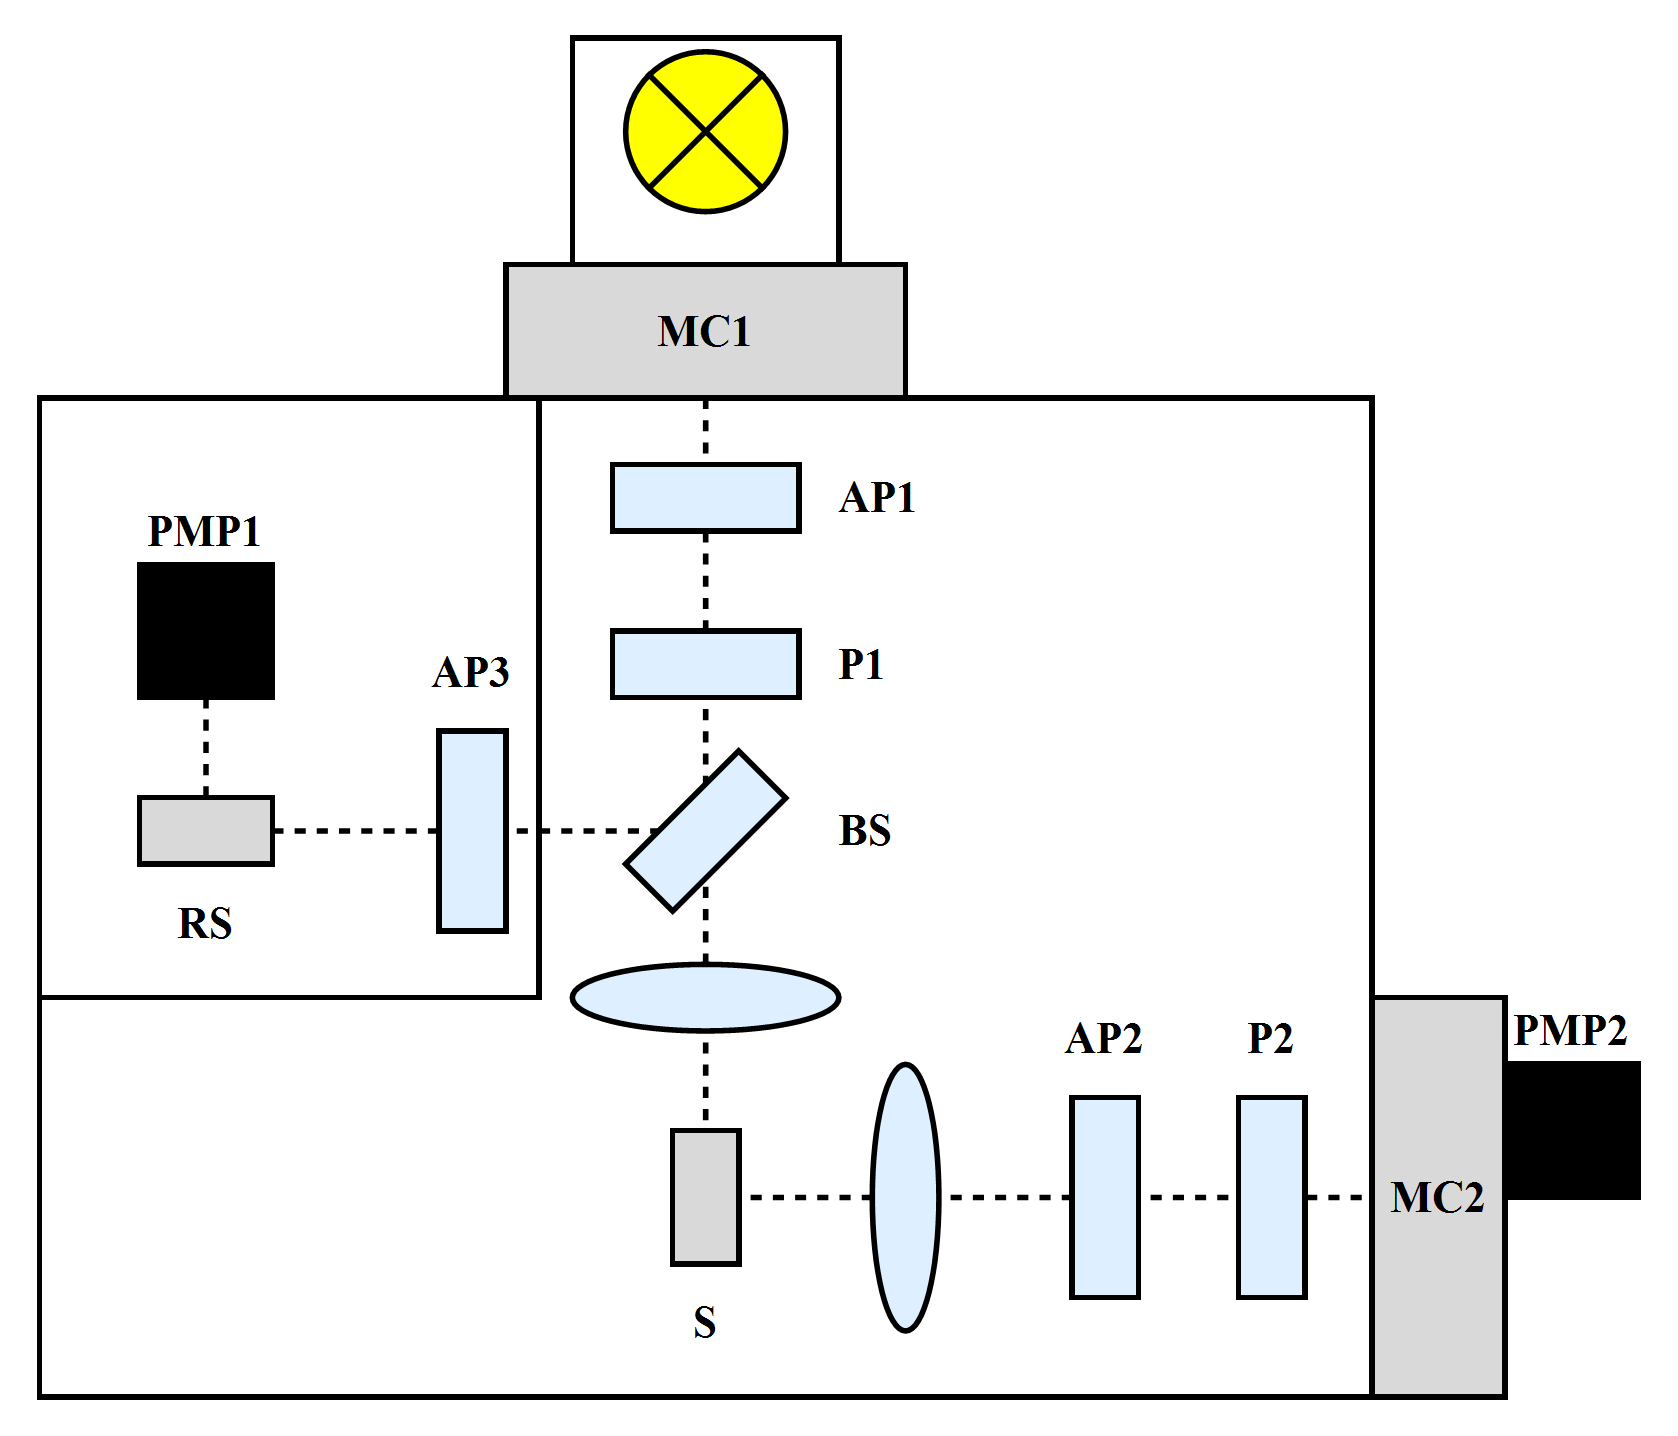
\includegraphics[width=0.55\linewidth]{img/setupStatic.png}}
\hfill
\subfloat[][Time Resolved Set-Up]{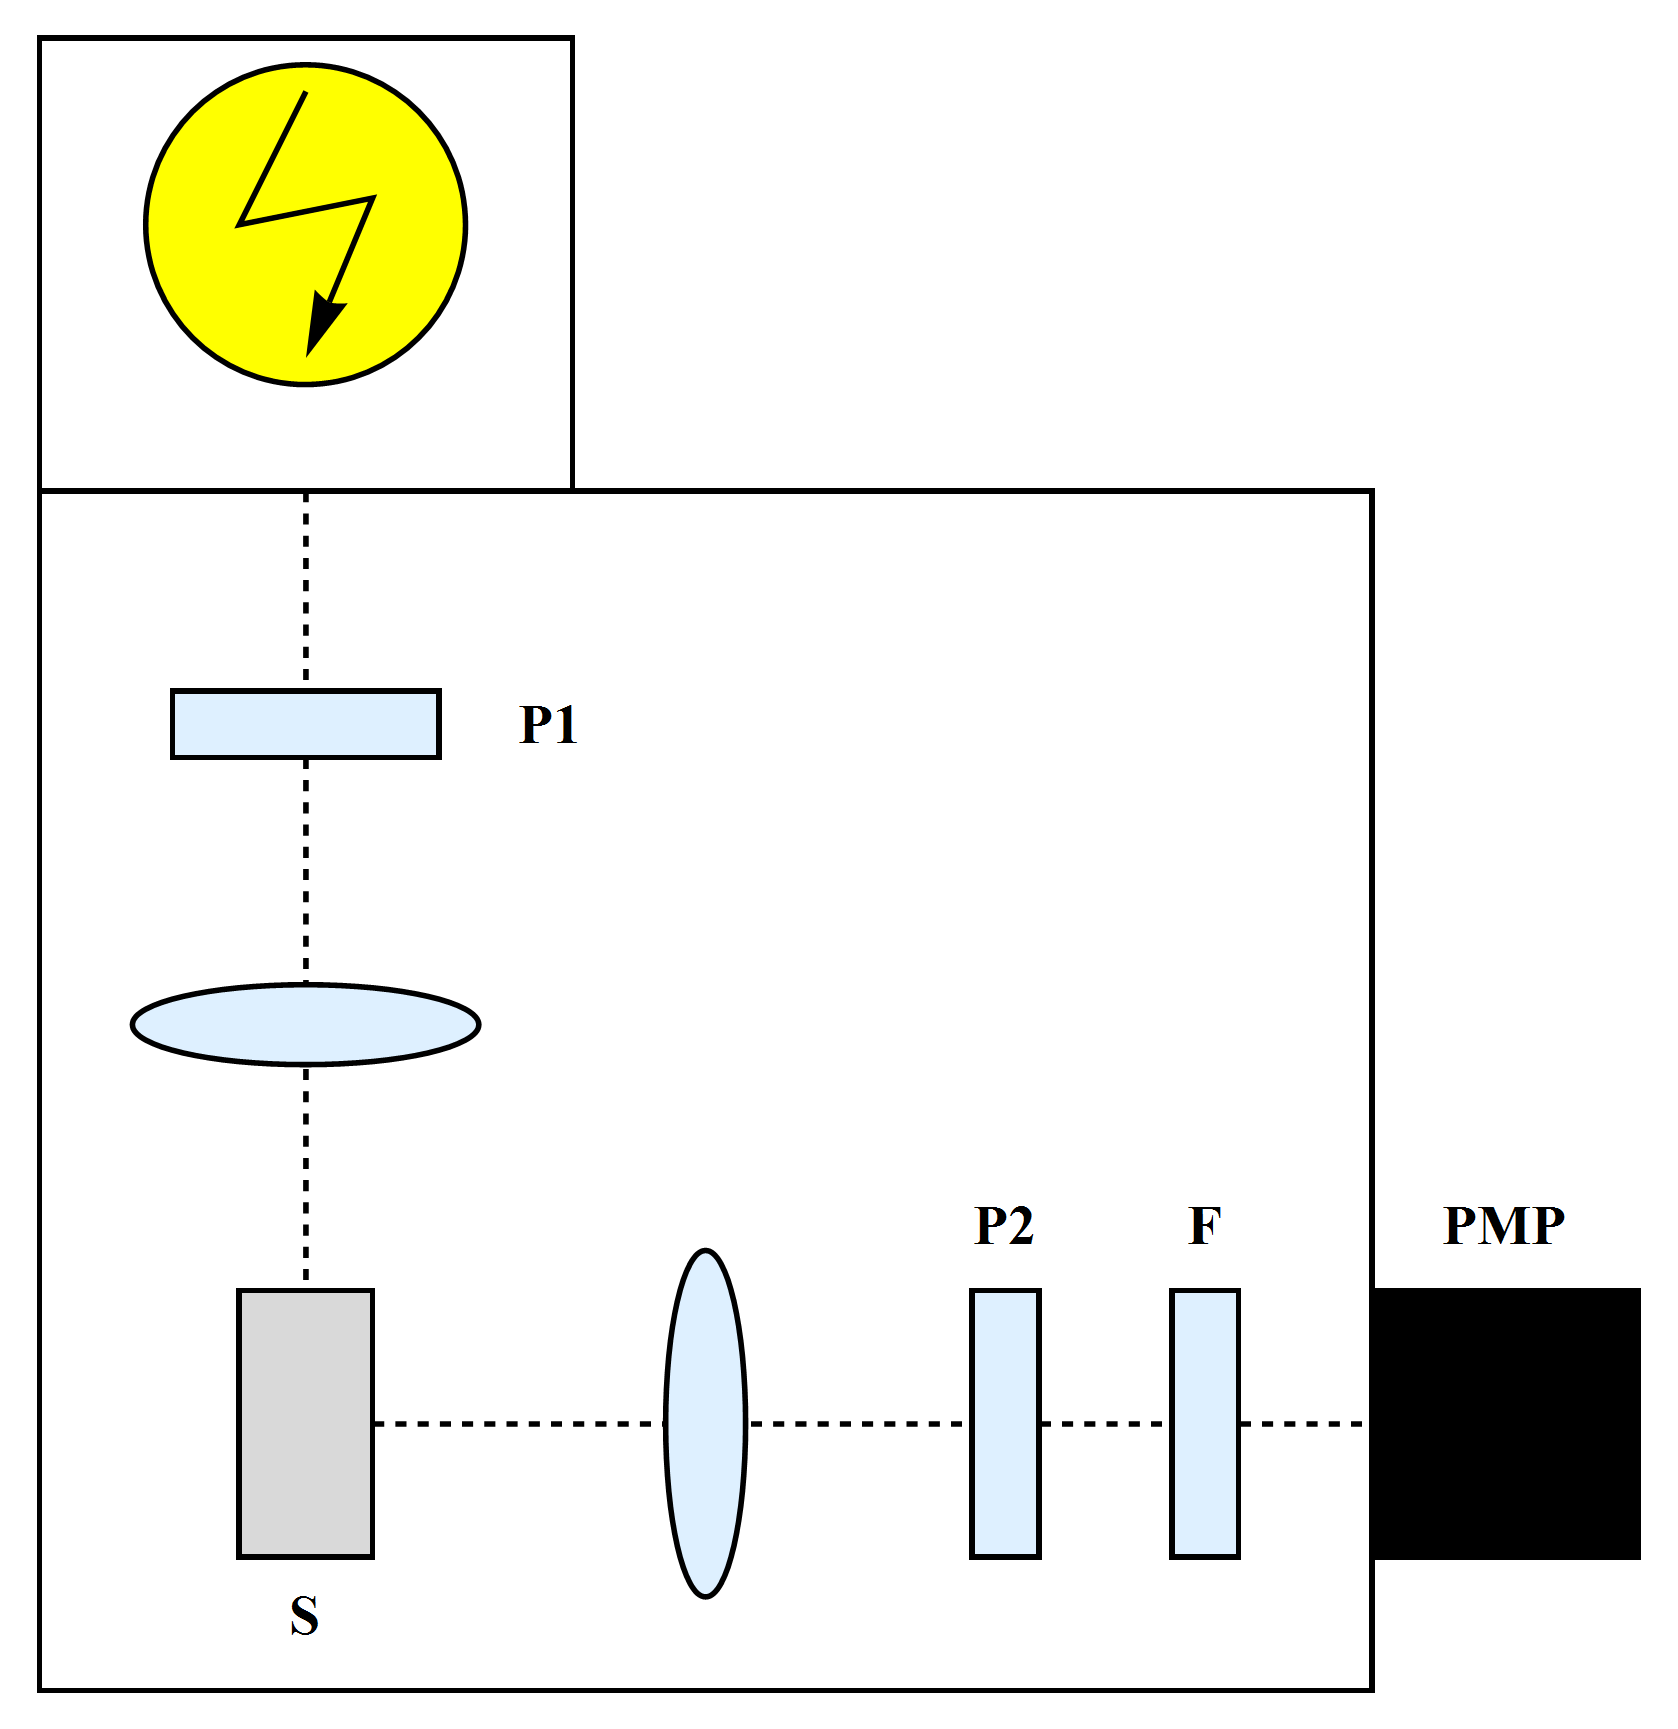
\includegraphics[width=0.45\linewidth]{img/setupDynamic.png}}
\caption{ \small \textbf{(a)} Set-Up for . \textbf{(b)} Set-Up for.}
\label{fig:setup}
\end{figure}

\subsection{Absorption and Emission Spectra}
The emission and absorption spectrum of a sample with \SI{8}{\micro l} \SI{1}{mM} DPH in THF in \SI{1}{ml} vesicle solution (A) is analyzed and compared with a sample of the same DPH-THF solution, but dissolved in a buffer solution and not in a vesicle solution (B). The measurement is performed with the steady-state set-up displayed in figure \ref{fig:setup} and explained above. The absorption spectrum of sample A is measured for excitation wavelength between $\lambda_\text{ex}=\SI{270}{nm} - \SI{420}{nm}$ at a fixed emission wavelength of $\lambda_\text{em}=\SI{450}{nm}$. The polarization filters are switched to vertical polarization to achieve highest intensity. The resolution of the spectrum is set to $\Delta \lambda =\SI{6}{nm}$ and the photomultipliers  are operated at: PM1 (sample) Range \SI{300}{nA}, Voltage \SI{13}{V}; PM2 (reference) Range \SI{3}{\micro A}, Voltage \SI{13}{V}.

The emission spectrum for sample A and B are recorded at an excitation wavelength of $\lambda_\text{ex}=\SI{360}{nm}$ for emission wavelength $\lambda_\text{ex}=\SI{380}{nm} - \SI{530}{nm}$ at the same operation parameters for the photomultipliers and polarization, except for the range of photomultiplier 1 (sample) that is changed to \SI{300}{nA} for the measurement of sample B, because the low intensity.

\subsection{Steady State Fluorescence Depolarization}
In order to investigate the phase transition of DMPC, the anisotropy $R$  is measured at different temperatures, that are induced by a heating machine, that heats up water, which floats around the sample. For each temperature and all four combinations of polarization filter configurations of the two polarizers five intensity values are recorded and the average value is used for the calculation of the anisotropy according to \Formel{R}. As the temperature can only be measured before and after each measurement, the values are recorded for the averaged temperature (before and after measurement).

\subsection{Time Resolved Fluorescence Depolarization}
The time-resolved fluorescence depolarization is performed with the second set-up. At first the flashlamp has to be filled with hydrogen, then a sample, that completely reflects light diffusive is inserted in order to measure the pure lamp function, which is later used to deconvolute the lamp signal from the measurement signal. For the time-resolution of the measurement a more-channel analyzator is used, which is triggered by the emission of a light pulse and then linearly increases a voltage. When a photon is detected it is stored into a channel coressponding to the voltage at this certain event-time. Therefore a calibration of the channel-number and the time is performed by setting four different time delays and comparing them to the channel number of highest intensity. The calibration yields $0.06849 \, \text{s}/\text{channel}$. Another calibration is made to determine the quantum yield of the photodetectors. To this end for a period of one minute the number of photons polarized horizontally and also the number of photons polarized vertically are counted (one after the other). The radio is determined to be $\Phi = 0.789$. 

For three different temperatures, 15 $\degree$ C,25 $\degree$ C and 38 $\degree$ C the intensity of light polarized horizontally and  are measured as a function of time in two different measurements. A computer program uses the intensity function of the lamp, as well as the two calibration parameters to process the measurement data and evaluate the anisotropy parameters by fitting exponential decay functions onto the anisotropy vs time.


\clearpage

\section{Analysis}


\subsection{Spectra}
Both, the absorption and the emission spectrum of the solution including the lipids, show the expected behaviour. They are similar in form, with four peaks each but mirrored at a point near 390\,nm (cf. figure \ref{fig:spectra}a-b).

\begin{figure}
\centering
\begin{tabular}{cc}
\subfloat[][absorption]{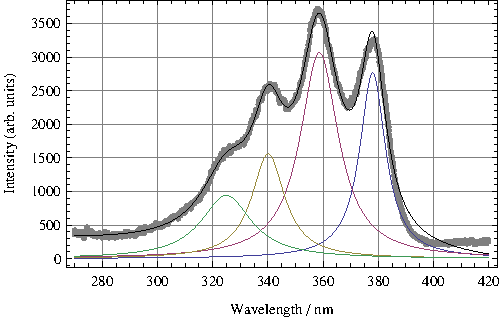
\includegraphics[width=0.47\linewidth]{img/abs.pdf}} &
\subfloat[][emission (vesicle)]{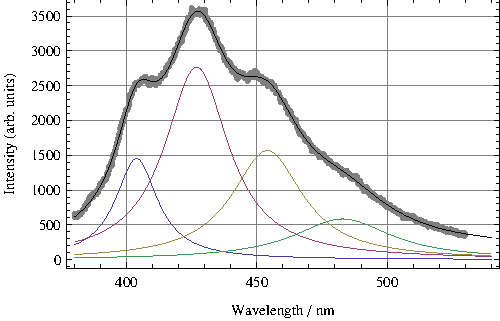
\includegraphics[width=0.47\linewidth]{img/emsves.pdf}} \\
\subfloat[][wavenumbers]{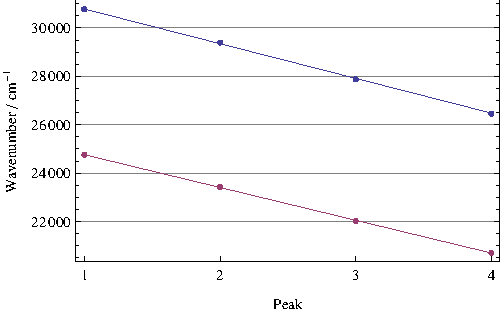
\includegraphics[width=0.47\linewidth]{img/peakwave.pdf}} &
\subfloat[][emission (water)]{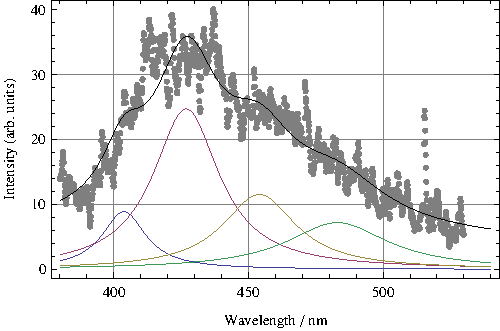
\includegraphics[width=0.47\linewidth]{img/emsnon.pdf}} \\
\end{tabular}
\caption{ \small Spectral measurements (gray) and their least-squares fits (black lines) as well as the four components of each fit that represent a single peak (colored). Peaks assumed to be of Gauß-Lorenzian shape with a linear noise function. \textbf{(a)} Absorptions spectrum with peaks at $(324.94\pm 0.57)\,\text{nm}$, $(340.14\pm 0.19)\,\text{nm}$, $(358.65\pm 0.09)\,\text{nm}$ and $(377.96\pm 0.07)\,\text{nm}$. \textbf{(b)} Emission spectrum with peaks at $(403.74\pm 0.07)\,\text{nm}$, $(426.86\pm 0.07)\,\text{nm}$, $(454.01\pm 0.14)\,\text{nm}$ and $(482.99\pm 0.62)\,\text{nm}$. \textbf{(c)} Peak positions from (a) and (b) converted to wavenumbers. The confidence intervals of all points are smaller than their markers in the plot. \textbf{(d)} Emission spectrum with DPH in a watery solution without lipids. For the fit the peaks are assumed to be at the same position and with the same FWHM as in (b). }
\label{fig:spectra}
\end{figure}

Assuming emissions at the same frequencies the emission rates of the sample without vesicles were fit as well to allow for a comparison of quantum yields (cf. figure \ref{fig:spectra}d). The ratio of the sums over all four peaks and thus the ratio of the quantum yields gives
\eq{\frac{\Phi(\text{DPH}_{H_2 O})}{\Phi(\text{DPH}_{\text{Lipid}})} = \frac{52.3\pm 1.7}{6367\pm 48} = (0.821\pm 0.027)\,\% . }{}
It can thus be approximated that all subsequent measurements of emissions are due to the DPH only without making an error of more than $0.8\,\%$.

Further information can be gained from the peak positions of the absorptions and emissions. Plotting the wavenumber against the number of the peak results in a linear dependency each. The two gradients are of further interest for us.
\eq{ \Delta E_{abs} = (1433\pm 22)\,\text{cm}^{-1} }{}
\eq{ \Delta E_{ems} = (1354.2\pm 9.3)\,\text{cm}^{-1} . }{}
As these are equal to the energy between two vibrational modes, the vibrational frequencies follow
\eq{ \omega_0 = \Delta E_{ems} / \hbar = (40.60\pm 0.28)\,\text{THz} }{}
\eq{ \omega_1 = \Delta E_{abs} / \hbar = (42.97\pm 0.64)\,\text{THz} . }{}
Or using the mass of carbon and the typical relations for harmonic oscillators for the amplitude $d=\sqrt{\hbar / (m\omega)}$ and for the force constant $k=m\omega^2$ we get
\eq{ d_0 = (32.87\pm  0.45)\,\text{pm} \qquad k_0 = (11.413\pm 0.039)\,\text{N\,m}^{-1}\;}{}
\eq{ d_1 = (36.82\pm  1.10)\,\text{pm} \qquad k_1 = (11.094\pm 0.083)\,\text{N\,m}^{-1} .}{}
The amplitude of the oscillation is small compared to the molecules length of approximately $13\,\AA$ and thus seems reasonable.

\clearpage

\subsection{Phase Transition of DMPC}
The fluorescence anisotropy measurements performed on the vesicle solution yields the data, which is plotted in figure \ref{fig:phase}. In order to determine the phase transition temperature the data is fitted with the model $R(T) = a_0 + a_1 T + a_2 \text{Erf}(T - T_c)$, where Erf is the Gaussian error function, expected to be a good approximation for the phase-transition region, $a_0$ is a constant height offset, $a_1$ is the slope of the two lines in the part excluding the phase-transition point, $a_2$ is the step-width of the error function and $T_c$ is the critical temperature. In principle the two lines can have different slopes, because the dependency of the anisotropy on temperature can be different in the two phases, however, the data is by far not precise enough to real such a feature. Plus, the slope of the low temperature region seems to reveal a descending tendency, which is unphysical. Therefore this possibility is not considered any further. The fit is performed according to the maximum likelihood methods, while the errors of each data point are given by the standard deviation of the five recorded values per point. The transition temperature is found to be
\eq{ T_C = ( 28.0 \pm 0.2 ) \, \degree \text{C} \; }{Tc}
and the slope left and right of the phase transition is $s = (-1.4 \pm 0.4 ) \cdot 10^{-3} / \degree \text{C}$. 

The van't Hoff enthalpy of the phase transition is given by the slope of $\Theta(T)=M1/(M1+M2)$, where $M1$ and $M2$ are determined by subtracting the respective asymptotic straight lines from the measurement data (cf. fig. \ref{fig:phase}). The slope is determined by fitting the model $\Theta(T)=a_0+a_1 \text{Erf}\left(a_2(T-T_c)\right)$, where $a_2$ allows for additional stretching and taking its derivative in the phase-transition region
\eq{\left. \frac{\mathrm d \Theta (T) }{\mathrm d T}\right|_{T=T_c} = (0.6 \pm 0.2) / \degree \text{C} \; .}{}
According to equation \Formel{dTheta} the van't Hoff enthalpy is
\eq{\delta H = 4 R T^2 \left. \frac{ \mathrm d \Theta (T) } {\mathrm d T}\right|_{T=T_c} = (1.8 \pm 0.7) \, \frac{ \text{MJ} }{ \text{Mole} } \; .}{}



\begin{figure}
\centering
\subfloat[][Anisotropy $R$]{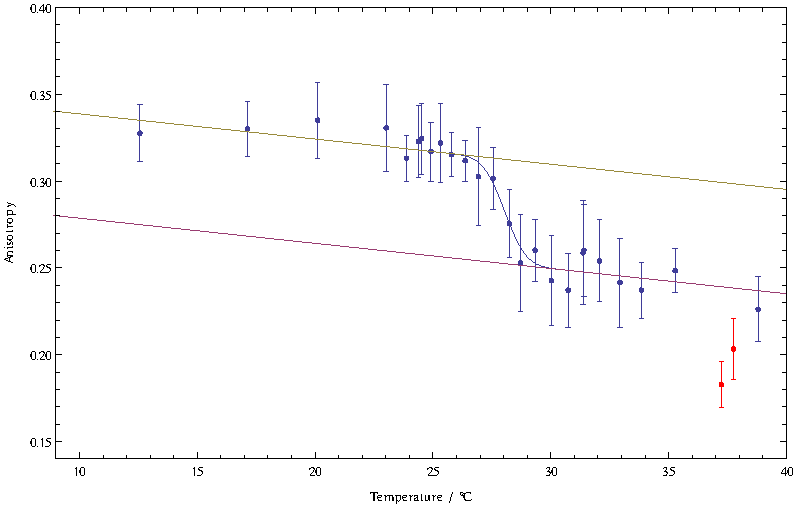
\includegraphics[width=\linewidth]{img/phasetransition.pdf}}

\subfloat[][Conversion Yield $\Theta$]{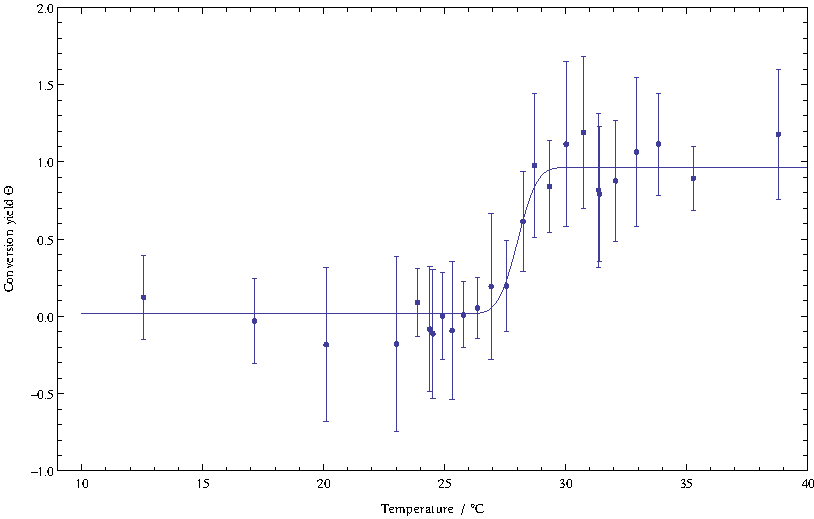
\includegraphics[width=\linewidth]{img/theta.pdf}}
\caption{ \small \textbf{(a)}Fluorescence anisotropy of a vesicle membrane (DMPC lipids) for different temperatures. At $T_C=28.0 \, \degree$ C an abrupt change of the anisotropy indicates a phase transition. The points marked in red are considered to be outliers and are ignored in the fit. \textbf{(b)} Conversion yield $\Theta$ as a function of temperature. From the slope at the phase transition temperature the van'T Hoff enthalpy can be calculated.}
\label{fig:phase}
\end{figure}

\clearpage

\subsection{Timeresolved Anisotropy}
The time dependence of the emitted light highly depends on the time dependence of the absorbed light flash. To account for this, the lamp signal was measured as well as the time dependence of the emissions (figure \ref{fig:aniTime}a). By deconvolution with the lamp signal, the actual time dependence (as it would be with a perfect flash) of emission can be approximated (figure \ref{fig:aniTime}b).

\begin{figure}
\begin{tabular}{cc}
\subfloat[][measured intensities at $15\,^\circ$C]{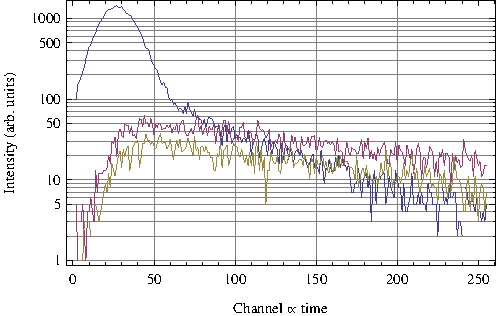
\includegraphics[width=0.47\linewidth]{img/4channel.pdf}} &
\subfloat[][anisotropy over time]{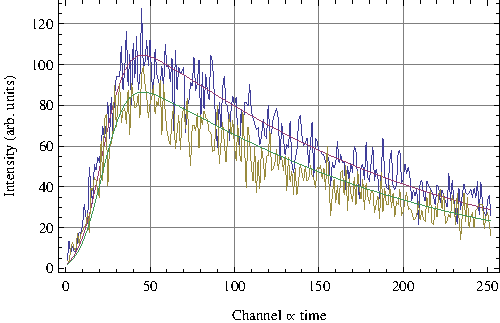
\includegraphics[width=0.47\linewidth]{img/twoT.pdf}} \\
\end{tabular}
\caption{\small \textbf{(a)} Measured time dependence of the light flash (blue) and the two polarizations at $15\,^\circ$C. \textbf{(b)} Deconvoluted intensity over time of the $25\,^\circ$C (blue, top) and $38\,^\circ$C (bottom) measurement as given by the program. The Deconvolution of the $15\,^\circ$C measurement was not saved by the program. }
\label{fig:aniTime}
\end{figure}

From these time dependencies a series of useful values can be calculated. Table \ref{tab:bla} lists these results as given by the program and the values for the diffusion constant, viscosity and cone opening angle as they result from these values.

Unfortunately the fits are rather bad. Several confidence intervals are much larger than their corresponding maximum likelihood value. $\Phi_\text{rot}$, $D$ and $\eta$ can thus not be evaluated further because only the last measurement of $38\,^\circ$C gave proper values for these. $R(0)$ is given without an error by the program, but especially the value for $25\,^\circ$C makes no sense at all. The other two values for $R(0)$ are rather large as well (should be around $0.3$). The expected behavior, that $R(0)$ is independent of the temperature can not even be confirmed.

\begin{table}
\centering
\rowcolors{1}{white}{gray!20}
\begin{tabular}{r|ccc}
T & $15\,^\circ$C & $25\,^\circ$C & $38\,^\circ$C \\
\hline
\hline
$\Phi_\text{rot} / \text{ns}$ & $0.14\pm 0.31$ & $0.06\pm 0.13$ & $0.25\pm 0.12$ \\
$R(0)$ & $0.7818$ & $1.854$ & $0.8147$ \\
$R(\infty)$ & $0.3022\pm 0.0082$ & $0.2029 \pm 0.0076$ & $0.1525 \pm 0.0088$ \\
$\langle R(T) \rangle_t$ & $0.3088\pm 0.0209$ & $0.2131\pm 0.0285$ & $0.1701\pm 0.0129$ \\
$\tau / \text{ns}$ & $9.76\pm 0.29$ & $9.19\pm 0.24$ & $9.03\pm 0.25$ \\
\hline
\hline
$D / \mu\text{s}^{-1}$ & $0.7\pm 1.7$ & $2.6\pm 5.7$ & $0.55\pm 0.25$ \\
$\eta / \text{Pa\,s}$ & $0.068\pm 0.155$ & $0.033\pm 0.072$ & $0.233\pm 0.116$ \\
$\theta / ^\circ$ & $43.77\pm 0.15$ & $62.95\pm 0.42$ & $56.22\pm 0.82$ \\
\end{tabular}
\caption{\small Rotational correlation times, anisotropy limits, time averaged anisotropy and decay rate as calculated by the software from the time resolved measurement. Diffusion constant $D$ and viscosity $\eta$ from equation (\ref{eq:diff}) using $V_\text{eff} f = (1.63\pm 0.34)\cdot 10^{-22}\,\text{cm}^3$ from \cite{heyn}, opening angle $\theta$ from equation (\ref{eq:theta}).  }
\label{tab:bla}
\end{table}

The derived value of the opening angle $\theta$ appears to have a very small error as we had to assume $R(0)$ to be without error (due to a lack of other data), but are just as questionable as the values of $R(0)$ themselves. Only by disregarding the value of the $25\,^\circ$C measurement we can see the expected trend of increasing opening angle with higher temperatures - but the unreliability of this data makes new measurements mandatory before drawing any conclusions.

At least the remaining values are realistic: $R(\infty)$ decreases with higher temperatures as expected, the mean values $\langle R(T) \rangle_t$ are in the range of previous measurements (though a bit smaller) and the decay times $\tau$ decrease with increasing temperature reflecting the higher mobility of molecules.

\section{Conclusion}
The method of polarization fluorescence spectroscopy was applied to investigate a lipid (DMPC) membrane vesicle solution. With the aid of a reporter molecule DPH, embedded in the membranes, rotational anisotropy measurements could be performed in steady-state and time-resolved experiments. 

The fluorescence absorption and emission spectrum of the vesicle solution is measured and fundamental molecule constants, such as the oscillation amplitude and the force constant are calculated resulting in reasonable values. The emission spectrum is furthermore compared to the one of a DPH sample without lipid vesicles. From the resulting quantum yield it is found, that the fluorescence emission of DPH is severely quenched in polar solutions.   

Steady-state fluorescence anisotropy was used to determine the phase transition temperature of DPMC molecules. The data showed high spread, which suggests some fundamental problem in the measurement set-up or defects in the sample. Some unexpected measurement values even proved to be reproducible. The phase transition temperature could however be determined quite well. Similar measurements by Heyn et al. \cite{heyn} gave a much lower transition temperature. This can be due to the fact, that the sample used in our measurement is probably quite old and the structure of the lipid membranes might have changed via the adsorption of solvent molecules or impurities brought into the sample through the opening of the cuvette, that is used in temperature measurements. The ratio of molecules, that have already gone through the phase transition divided by the total molecule amount participating in fluorescence, the so called conversion yield is calculated as a function of temperature and yields the van't Hoff enthalpy, which is by far larger than the ones measured by Heyn et al. \cite{heyn}. This is however not very surprising, as also the transitions temperature is very different and it is most probable, that the physical processes of the phase transition differs a lot. The van't Hoff enthalpy determined from calorimetric measurements yields much lower values, which would have probably also been the case for our sample This can be understood in terms of the so called cooperativity, which is a measure of how one phase transitioned molecule influences the phase transition properties of the surrounding molecules. The ratio of the van't Hoff enthalpies gained by the two different measurement methods yields the size of the cooperative unit cell, which is the number of molecules that tend to undergo a phase transition simultaneously rather than one by one. In order to make any more sensible statements on that, it would be necessary to perform a calometric measurement on exactly that sample or to provide a new sample, which is comparable to the work of Heyn et al..

The time-resolved fluorescence anisotropy measurement was performed for three different temperatures in order to determine the rotational correlation times, the anisotropy in the limit of zero time and infinite time, as well as the average anisotropy and the decay rate. Furthermore the diffusion constant, the viscosity and the opening angle were calculated within the frame-work o the wobbing-in-cone model. The measured rotational correlation times, the anisotropy at time zero, the diffusion constant and the opening angle are unphysical as they do not show the expected temperature dependence and have exceedingly large measurement errors. Therefore, no significant information can be extracted from the latter. However the rotational anisotropy in the infinite time limes, as well as the mean anisotropy values and the decay rate meet the expected temperature dependence and agree with the measurements in the steady state experiment.








 \bibliographystyle{unsrt}
\bibliography{bib}



\end{document}


